\section{Water Models}\label{sec:water_models}

% Navier stokes, Different level of water depth, Spatial, Spectral domain,
% eulerian, lagrangian frameworks, talk about their visual accuracy, SLProject,
% 0 a.d.

% Talk about the different depth of water

We start this section by presenting the physically accurate description of
fluids, \nameref{subsec:navier_stokes}, in \autoref{subsec:navier_stokes}. Water
models are separated into groups depending on the water depth: deep,
intermediate or shallow. This classification takes its root from oceanography
\autocite{darles2011survey}. We will present the deep water group in
\autoref{subsec:deep_water} and the shallow one in
\autoref{subsec:shallow_water} (we include the intermediate models directly into
the shallow group). For each of them we will present selected relevant
approaches from the literature. These two groups describe only the
\textit{shape} of the water. In \autoref{subsec:ocean_details} we discuss the
methods to produce realistic water surfaces. This includes caustics, foam, light
scattering and more. Finally in \autoref{subsec:candidate_apps} we talk about
two applications in need of a real-time water solution. Readers who desire to
get a broader picture about water rendering should read the survey from
\citeauthor{darles2011survey} \autocite{darles2011survey}.


\subsection{Navier-Stokes Equations}\label{subsec:navier_stokes}

% explain that they describe a fluid but they don't have a solution yet and it's
% one of the biggest open problems in math. Computational Fluid Dynamics CFD is
% the field of finding numerical approximations to the equations
% The process of solving problems in fluid dynamics numerically on a computer is
% called CFD

Navier-Stokes Equations (or NSE) describe the motion of a fluid in any dimension
$\mathbb{R}^n$. They are named after Sir George Gabriel Stokes\footnote{Best
known for \textit{Stokes's law}, the expression of the frictional force of a
fluid exerted onto a sphere.}, an Irish mathematician and physicist and Henri
Navier, a French engineer, mathematician and economist. Both worked on, and
enhanced the Euler equations. Navier proposed in 1820 to add a term to them for
the heat dissipation. In 1845 Stokes also suggested introducing a term for the
energy dissipation in form of heat \autocite{gallagher2010autour}. The equations
are shown below only for the curious reader as we will not further discuss them.
The Navier-Stokes equation of an incompressible fluid flow is:

\begin{equation}\label{eq:nse}
    \frac{\partial \textbf{u}}{\partial t} + \textbf{u}\cdot \nabla \textbf{u}
     = - \frac{\nabla P }{\rho} + \nu {\nabla}^2 \textbf{u}
\end{equation}
%
where $\nu$ is the kinematic viscosity, $\textbf{u}$ is the velocity of the
fluid parcel, $P$ is the pressure, $\rho$ is the fluid density and $t$ the
time \autocite{weisstein2018navier}.

Solving the Navier-Stokes equations in three dimensions remains an open problem
in mathematics and physics. It is one of the seven ``Millennium Problems''
defined by the Clay Mathematics Institute.

We felt the need to mention them here because all the water models found in the
literature are somehow linked to them. Computational Fluid Dynamics (CFD) is the
field of finding numerical approximations to those equations. 


\subsection{Deep Water Models}\label{subsec:deep_water}
% What is the spatial domain?  present some papers:
% - Johanson
% What is the spectral domain?  present some models in the spectral and spatial
% domains from different papers that look great:
% - Tessendorf
% - GPU Gems 2 Effective Water Simulation from Physical Models
% - Using Vertex Texture Displacement for Realistic Water Rendering
Deep water models can further be classified into two groups: spatial and
spectral \autocite{darles2011survey}. To describe the water surface the former
uses a sum of sines and cosines and the latter an inverse fast Fourier transform
(IFFT)\footnote{The FFT approach allows to use data from a buoy or from aerial
water photographs.}. Unfortunately both have downsides: spatial models produce
water having a too rounded shape and spectral models are difficult to control
\autocite{darles2011survey}. In order to benefit from both, a hybrid solution
should be chosen \autocite{darles2011survey}. We present two models: one for
each group.

%\subsubsection{Projected Grid Concept}
\subsubsection{Gerstner Waves}\label{subsub:gerstner}
%\subsubsection{Vertex Texture Displacement}

Observing the ocean from the atmosphere, as seen in figure
\autoref{fig:barren_island}, a slightly repetitive pattern is noticeable. This
resembles strongly to a hevily disturbed combination of sines and cosines. The
combination of such curves, also called \textit{Gerstner
Waves}\footnote{Gerstner Waves where first described in
\autocite{gerstner1802theorie} and provide a solution to a certain type of
Euler equations.}, was proposed in \autocite{max1981vectorized} for their
ray-tracing procedural model. The height $y = h(x,z,t)$ for each point $(x,z)$
at time $t$ is

\begin{equation}\label{eq:gerstner_max}
    h(x, z, t) = -y_0 + \sum_{i = 1}^{N_w} A_i \cos(k_{i_x}x + k_{i_y}y -
    \omega_i t)
\end{equation}
%
where $N_w$ is the total number of waves, $A_i$ is the amplitude of wave $i$,
$(k_{i_x}, k_{i_y})$ the wave vector and $\omega_i$ the angular frequency
\autocite{max1981vectorized,darles2011survey}. \autoref{fig:max_raytraced}
depicts the sum of four such waves rendered in 1981.

\begin{figure}[hbt!]
    \centering
    \begin{subfigure}[hbt]{\textwidth}
        \centering
        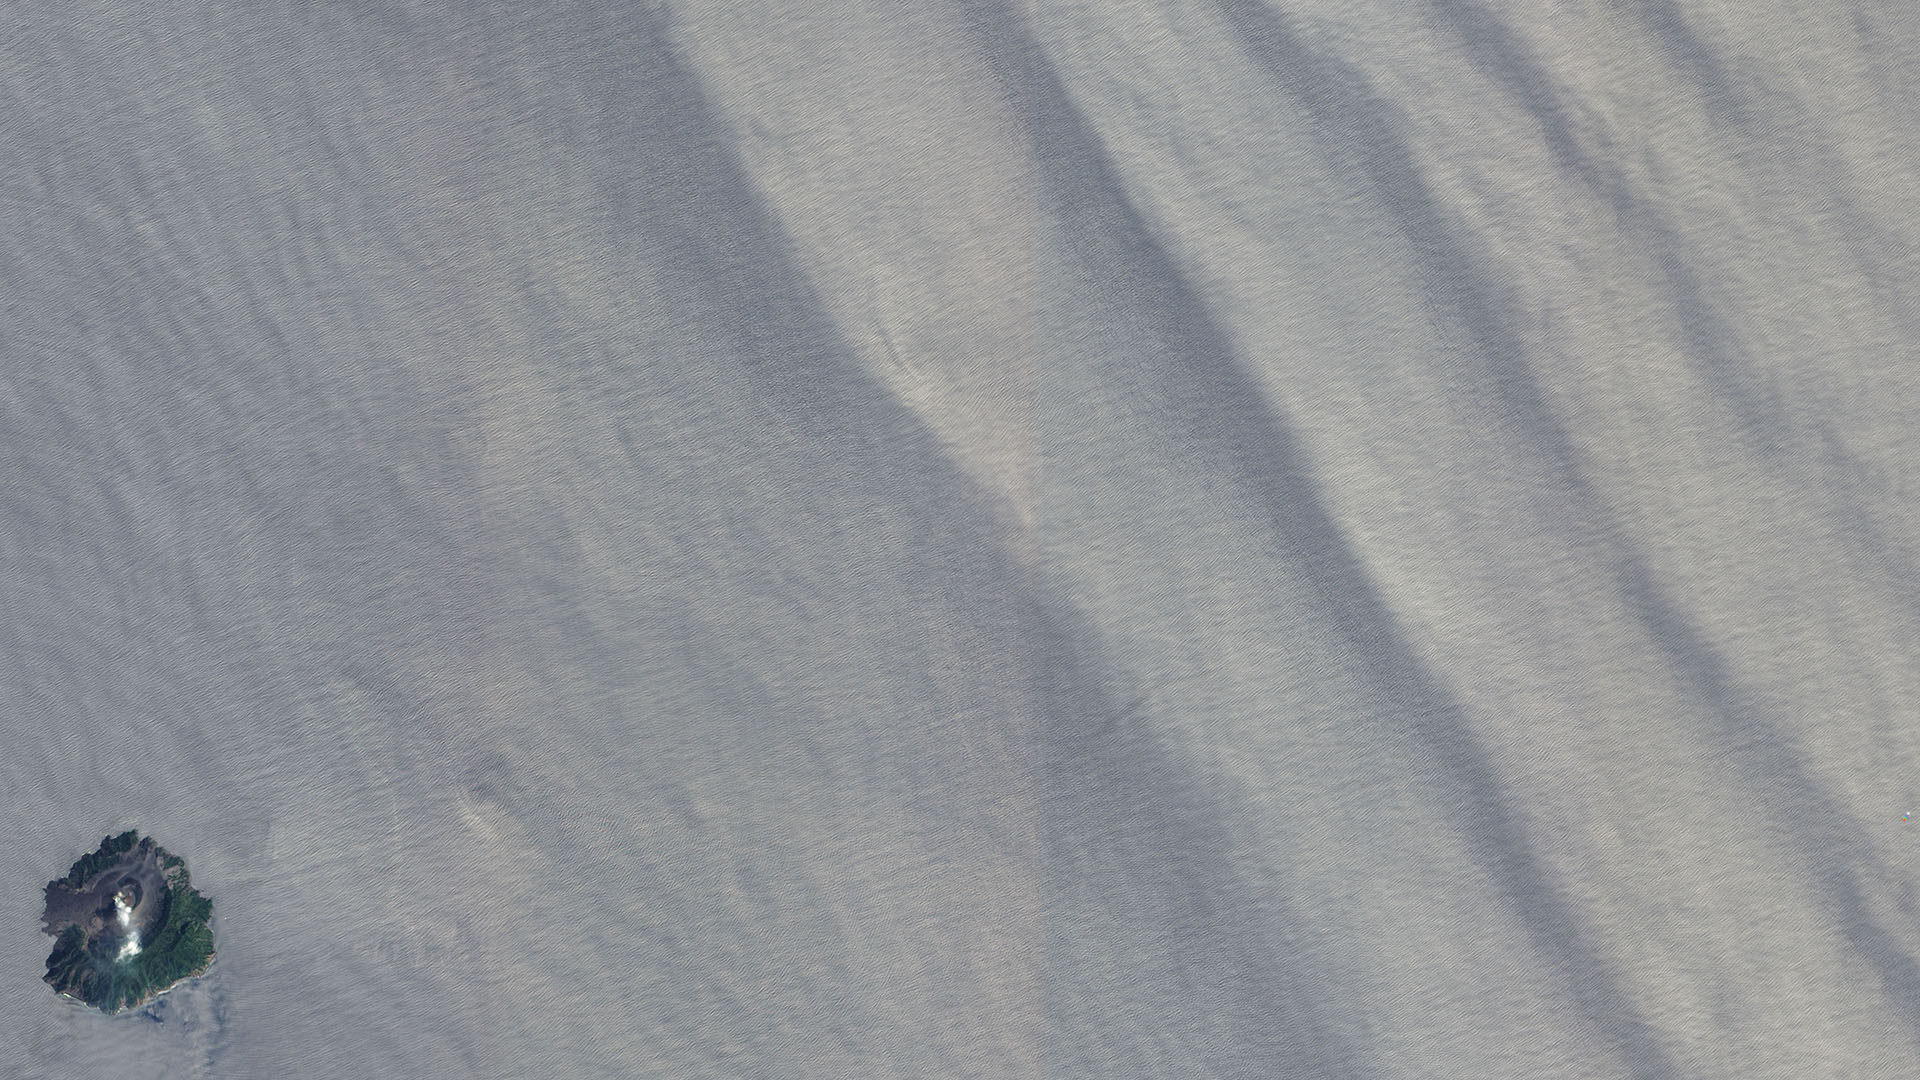
\includegraphics[height=5cm]{barren_island_far.jpg}
        \subcaption{Far view of the Barren
        Island}\label{subfig:barren_island_far}
    \end{subfigure}\\%
    %  
    \begin{subfigure}[hbt]{\textwidth}
        \centering
        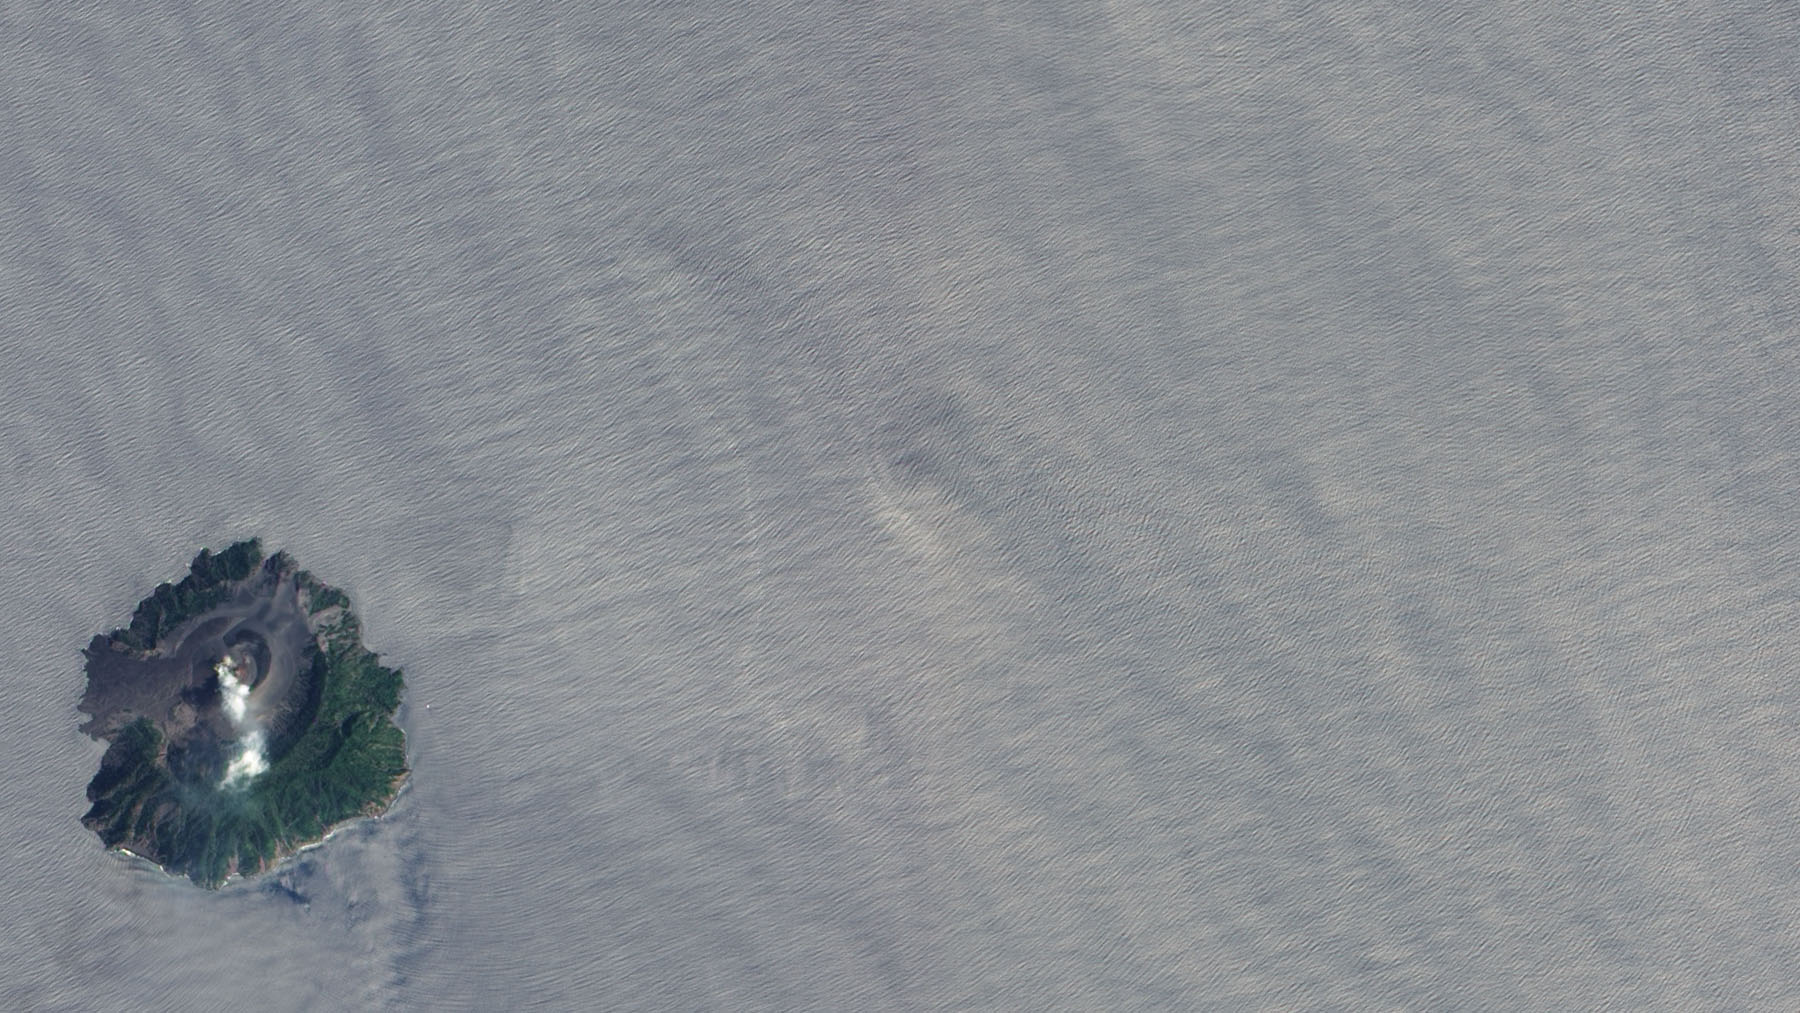
\includegraphics[height=5cm]{barren_island_close.jpg}
        \subcaption{Close view of the Barren
        Island}\label{subfig:barren_island_close}
    \end{subfigure}
    \caption{The Barren Island captured by the Earth Observing-1 satellite in
        2007. The darker waves in \autoref{subfig:barren_island_far} are
        deep internal waves (source:
        \url{earthobservatory.nasa.gov}).}\label{fig:barren_island}
\end{figure}

\begin{figure}[hbt]
    \centering
    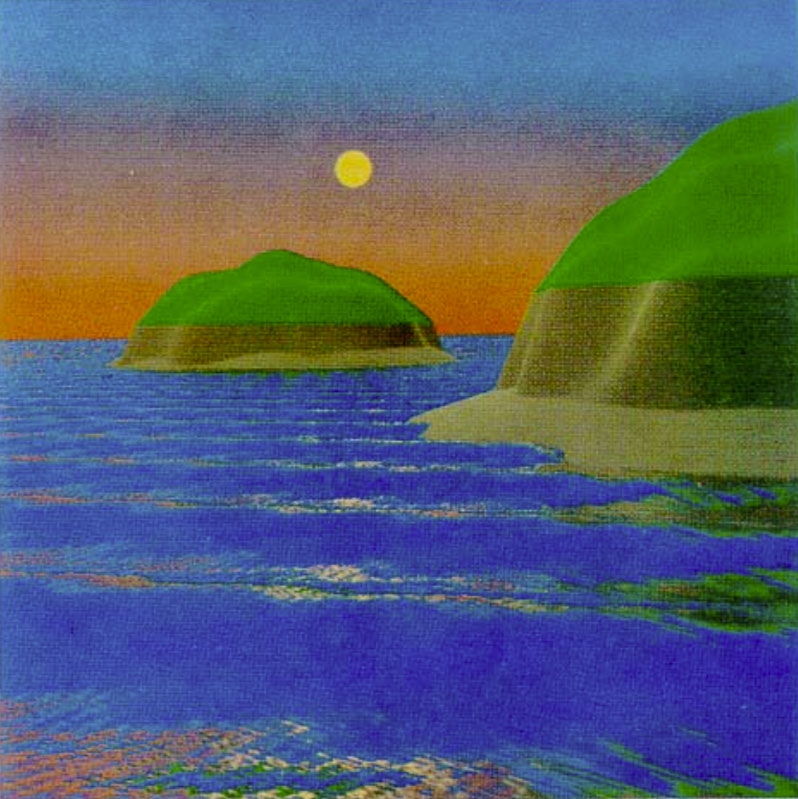
\includegraphics[height=5cm]{max1981raytracing.jpg}
    \caption{Ray-tracing of four waves using \autoref{eq:gerstner_max}. Source:
    \autocite{max1981vectorized}}\label{fig:max_raytraced}
\end{figure}

Another form of recommended Gerstner Waves, described in
\autocite[Chapter~1]{fernando2004gpu}, displaces also the $x$ and $z$
directions. $\textbf{P}$ is the position in space, and $\textbf{N}$ is its
corresponding normal. See \autoref{eq:gerstner_position} and
\autoref{eq:gerstner_normal}.

\begin{equation}\label{eq:gerstner_position}
    \textbf{P}(x,y,t)=\begin{bmatrix}x\\ y\\ z\end{bmatrix}=\begin{bmatrix} x +
    \sum_{i}(Q_i A_i\cdot\textbf{D}_i.x\cdot \cos(\omega_i \textbf{D}_i\cdot
    (x,y) + \varphi_i t))\\ y + \sum_{i}(Q_i A_i\cdot\textbf{D}_i.y\cdot
    \cos(\omega_i \textbf{D}_i\cdot (x,y) + \varphi_i t))\\ \sum_{i}(A_i\cdot
\sin(\omega_i \textbf{D}_i\cdot (x,y) + \varphi_i t))\\\end{bmatrix}
\end{equation}

\begin{equation}\label{eq:gerstner_normal}
    \textbf{N}(x,y,t)=\begin{bmatrix}x\\ y\\ z\end{bmatrix}=\begin{bmatrix}
    - \sum_{i}(\textbf{D}_i.x\cdot WA \cdot C(\cdot))\\ 
    - \sum_{i}(\textbf{D}_i.y\cdot WA \cdot C(\cdot))\\ 
    1-\sum_{i}(Q_i \cdot WA \cdot S(\cdot))\\\end{bmatrix}
\end{equation}
%
With the substitutions $WA = \omega_i A_i,\ S(\cdot) = \sin(\omega_i
\textbf{D}_i \cdot \textbf{P} + \varphi_i t),\ C(\cdot) = \cos(\omega_i
\textbf{D}_i \cdot \textbf{P} + \varphi_i t)$.

The authors derive the binormal and tangent vectors from the position. They can
be used with the normal vector from \autoref{eq:gerstner_normal} to compute the
transformation from the tangent space into the local space.

\begin{equation}\label{eq:gerstner_binormal}
    \textbf{B}(x,y,t)=\begin{bmatrix}x\\ y\\ z\end{bmatrix}=\begin{bmatrix}
    1 - \sum_{i}(Q_i \cdot \textbf{D}_i.x^2 \cdot WA \cdot S(\cdot))\\
    - \sum_{i}(Q_i \cdot \textbf{D}_i.x \cdot \textbf{D}_i.y\cdot WA \cdot
    S(\cdot))\\ 
    \sum_{i}(\textbf{D}_i.x \cdot WA \cdot C(\cdot))\\\end{bmatrix}
\end{equation}

\begin{equation}\label{eq:gerstner_tangent}
    \textbf{T}(x,y,t)=\begin{bmatrix}x\\ y\\ z\end{bmatrix}=\begin{bmatrix}
    - \sum_{i}(Q_i \cdot \textbf{D}_i.x \cdot \textbf{D}_i.y\cdot WA \cdot
    S(\cdot))\\
    1 - \sum_{i}(Q_i \cdot \textbf{D}_i.y^2 \cdot WA \cdot S(\cdot))\\
    \sum_{i}(\textbf{D}_i.y \cdot WA \cdot C(\cdot))\\\end{bmatrix}
\end{equation}

The Gerstner wave approach is easy to implement and understand but produces too
rounded shapes. On one hand computing only four waves produces a too repetitive
result. On the other hand adding more of them reduces the performance. To obtain
a reasonable result it should be combined with another model.

\subsubsection{Fast Fourier Transform (FFT)}\label{subsub:fft}


The fast Fourier transform approach was introduced in 1987 by
\citeauthor{mastin1987fourier} \autocite{mastin1987fourier}. The representation
of the wave height $h$ given a horizontal position $\textbf{x} = (x,z)$ and the
time $t$ is given by

\begin{equation}
    h(\textbf{x}, t) = \sum_{\textbf{k}}^{} \tilde{h}(\textbf{k},
    t)e^{i\textbf{k}\cdot\textbf{x}}
\end{equation}
%
where $\textbf{k}$ is the wave vector and $\tilde{h}(\textbf{k}, t)$ is the
amplitude and phase of the $\textbf{k}$th wave at time $t$. The wave vector
$\textbf{k}$ is a two dimensional vector equal to $(k_x, k_z) = (2\pi n/s, 2\pi
m / s)$. $n$ and $m$ are bounded by the resolution $r$ of the grid in the
following manner: $-r/2 \leq n,m \leq r/2$. $s$ is the dimension of the animated
area \autocite{jensen2001deep,darles2011survey}.

In order to compute $\tilde{h}$ its value at time $t=0$ is needed, which is
denoted by $\tilde{h}_0(\textbf{k})$. Then $\tilde{h}(\textbf{k}, t)$ can be
expressed as

\begin{equation}
    \tilde{h}(\textbf{k}, t) = \tilde{h}_0(\textbf{k}) e^{i\omega(k)t} +
    \tilde{h}_0^*(\textbf{k}) e^{i\omega(k)t}
\end{equation}
%
where $\tilde{h}_0^*(\textbf{k})$ is the complex conjugate s.t.
$\tilde{h}(\textbf{-k})=\tilde{h}^*(\textbf{k})$ and $\omega(k)=gk$ with $g$
being the gravitational constant.

\citeauthor{mastin1987fourier} take for $\tilde{h}_0$ the following:

\begin{equation}
    \tilde{h}_0(\textbf{k}) = \frac{\alpha g^2}{{(2\pi)}^4 f^5}
    e^{-\frac{5}{4}{(\frac{f_m}{f})}^4}, \quad f_m=\frac{0.13}{u_{10}}
\end{equation}
%
$f$ is the frequency in Hz, $f_m$ is the peak frequency of the wind speed
$u_{10}$, measured at ten meters above the ocean surface, $\alpha=0.0081$ is
Phillips' constant and $g$ is again the gravitational constant.

\citeauthor{tessendorf2001simulating} proposed another amplitude function
$\tilde{h}_0$, 

\begin{equation}\label{eq:tessendorf_h0}
    \tilde{h}_0(\textbf{k}) = \frac{1}{\sqrt{2}}(\xi_r +
    i\xi_i)\sqrt{P_h(\textbf{k})}
\end{equation}
%
where $\xi_r$ and $\xi_i$ are constants and $P_h(\textbf{k})$, the spectrum, is:

\begin{equation}
    P_h(\textbf{k}) = A\frac{e^{\frac{-1}{{(kL)}^2}}}{k^4}
    |\textbf{k}\cdot\textbf{w}|
\end{equation}
%
$A$ is a constant, $L=V^2/g$, with $V$ being the wind speed, $g$ the
gravitational constant and finally $\textbf{w}$ the wind direction.

As seen in figure \autoref{subfig:fft_round}, the method only produces rounded
waves. In order to get the choppy effect of a stormy ocean, the position can be
displaced locally in the horizontal direction. This can be done with

\begin{equation}
    \textbf{x} = \textbf{x} + \lambda \textbf{D}(\textbf{x}, t), \quad
    \textbf{D} = \sum_{\textbf{k}}^{} -i\frac{\textbf{k}}{k}
    \tilde{h}(\textbf{k},t) e^{i\textbf{k}\cdot\textbf{x}}
\end{equation}

\begin{figure}[hbt!]
    \centering
    \begin{subfigure}[hbt]{0.45\textwidth}
        \centering
        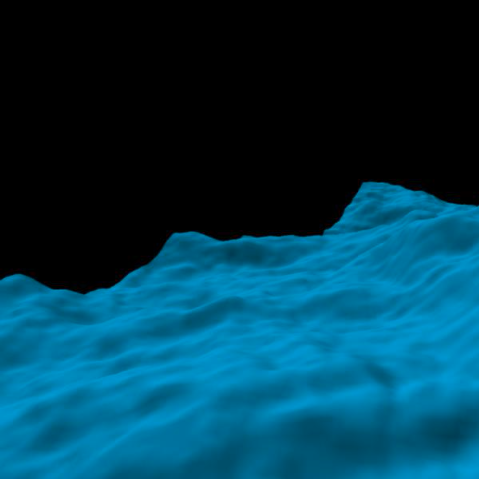
\includegraphics[height=4cm]{fft_rounded.png}
        \subcaption{Without local displacement}\label{subfig:fft_round}
    \end{subfigure}~%
    %  
    \begin{subfigure}[hbt]{0.45\textwidth}
        \centering
        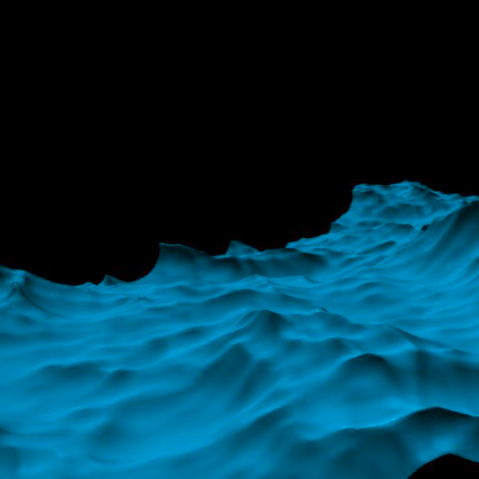
\includegraphics[height=4cm]{fft_sharp.png}
        \subcaption{With local displacement}\label{subfig:fft_sharp}
    \end{subfigure}
    \caption{Result from the use of the fast Fourier transform to compute the
    ocean's shape. Source:
    \autocite{tessendorf2001simulating}.}\label{fig:fft_comparison}
\end{figure}

Using this method, it is possible to compute two height fields of different
resolution. The first one can be used as a displacement map and the second one
as a bump map. As already mentioned before, the frequency spectrum is hard to
control for an artist and the gird needs to be large to display most of the
frequencies \autocite{gonzalez2016rendering}.


%\subsubsection{Hybrid}

\subsection{Shallow Water Models}\label{subsec:shallow_water}

Shallow water models try to discretize the Navier-Stokes equations (described in
\autoref{eq:nse}) in two ways \autocite{darles2011survey}. The first one uses a
two or three dimensional grid to represent the fluid moving from cell to cell.
It is called the Eulerian approach. The second one makes the assumption that
particles transport a small fluid volume. This one is called the Lagrangian
approach. Both share similar problems and advantages
\autocite{darles2011survey}. The two can reproduce many different phenomena but
are constrained by the grid size and the particle amount. They also become
expensive when simulating finer details such as foam and spray as they need a
lot of cells or particles \autocite{darles2011survey}.

We will present only one hybrid method because a derivation of it has been used
for an industry production as described in \cref{subsub:uncharted}.

\subsubsection{Wave Particles}\label{subsub:wave_particles}
% Combines the Eulerian approach for the shape and the Lagrangian approach for
% interaction with the water.
% Also include object interaction. The waves are generated with a height field.
% The object interaction is done with vertical cells. Depending whether the
% object pushes into the water or pulling out of the water they generate a wave
% with a negative, respectively positive amplitude moving away from the object.
% Moving away only if the object is not fully submerged. If it is they move
% towards the object.
% Each face of the object is handled differently.
% Only focuses on surface waves.
% Does not generate waves.

The \textit{Wave Particles} method as described in \autocite{yuksel2007wave} is
a hybrid shallow water model. It uses an Eulerian approach to compute the shape
of the water and a Lagrangian one for the interaction with objects. Each
\textit{particle} is subdivided into three smaller ones as the wave expands. If
the \textit{particle} is too small it dies and is not displayed. When a
\textit{particle} encounters a fixed boundary it is reflected back. To compute
the water volume moved by an object, \citeauthor{yuksel2007wave} find the volume
displaced by each face of the object. This is done with the help of a low
resolution silhouette in form of a texture. They also compute the buoyant, drag
and lift forces acting on the object \autocite{yuksel2007wave}. The result can
be seen in \cref{subfig:wave_particle_1,subfig:wave_particle_2}.

\begin{figure}[hbt!]
    \centering
    \begin{subfigure}[hbt]{\textwidth}
        \centering
        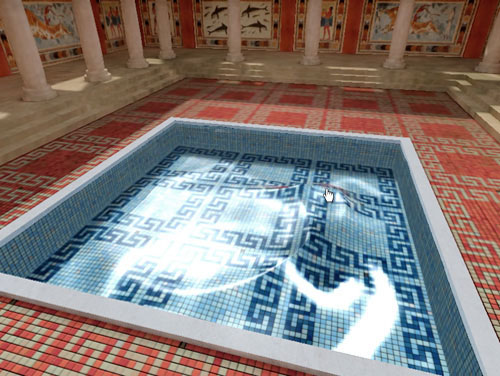
\includegraphics[height=5cm]{wave_particle_1.jpg}
        \subcaption{Pool test scene, source
        \autocite{yuksel2007wave}}\label{subfig:wave_particle_1}
    \end{subfigure}\\%
    %  
    \begin{subfigure}[hbt]{\textwidth}
        \centering
        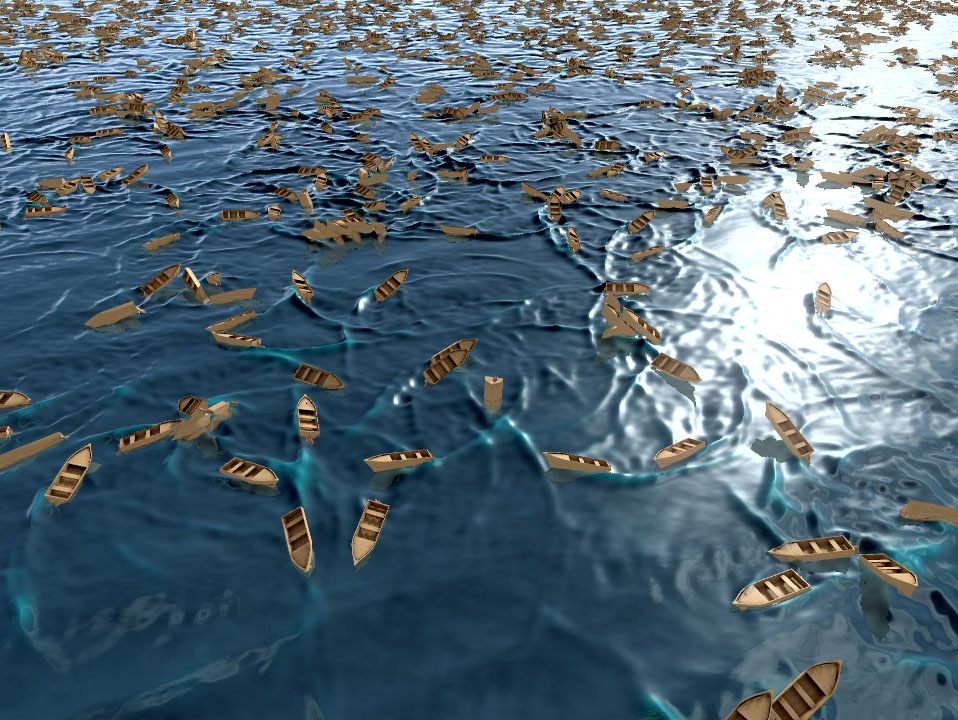
\includegraphics[height=5cm]{wave_particle_2.jpg}
        \subcaption{Boat armada test scene, source
        \autocite{yuksel2007wave}}\label{subfig:wave_particle_2}
    \end{subfigure}
    \caption{Result of the demonstration application from
    \autocite{yuksel2007wave}}\label{fig:wave_particle}
\end{figure}

\subsection{Rendering of Ocean Details}\label{subsec:ocean_details}
% Modeling waves and surf 1986
% Nishita et al. [NSTN93] Check the ocean color part
% Also check On Modeling and Rendering Ocean Scenes
% A Procedural Model for Interactive Animation of Breaking Ocean Waves
% Towards Real-Time Visual Simulation of Water Surfaces
% Realistic Water Volumes in Real-Time
% Rendering Natural Waters
% GPU-based Ocean Rendering

% Talk about reflection, refraction, foam, splash, caustics, color of the water

Up until now we only presented methods which describe the shape of the water.
The most important property of water is its reflection and refraction. We will
discuss those two in \cref{subsub:reflection_refraction}. Closely linked to them
are caustics (\cref{subsub:caustics}). Another one which can be observed is
foam, presented in \cref{subsub:foam}. Finally the color of the water varies
depending on the environment as explained in \cref{subsub:caustics}.

\subsubsection{Reflection and Refraction}\label{subsub:reflection_refraction}

Reflection can occur on any kind of surface. The most common one encountered
every day is the mirror. The law of reflection states that the angle of
incidence between the normal and an incident ray is equal to the angle between
the normal and the reflected ray. The reflection vector can be computed using
\autoref{eq:reflection}. A visual representation can be seen in
\autoref{fig:reflection}.

\begin{equation}\label{eq:reflection}
    \textbf{r}_{i} = \textbf{l} - 2(\textbf{l} \cdot
    \textbf{n})\textbf{n}
\end{equation}

Refraction depends on the two media the incident ray interacts with, as shown in
\autoref{fig:reflection_refraction}. It follows Snell's law from
\autoref{eq:snell}. 

\begin{equation}\label{eq:snell}
    \frac{\sin(\theta_i)}{\sin(\theta_t)} ={} \frac{n_t}{n_i}
\end{equation}

To get the refraction vector, we need to use \autoref{eq:snell} and split up
$\textbf{t}$ into its tangent and normal part. The result is shown in
\autoref{eq:refraction}.

\begin{equation}\label{eq:refraction}
    \textbf{t} = \frac{1}{n} \textbf{l} +
    \left(\frac{1}{n}\cos(\theta_i) + \sqrt{1 - \frac{1}{n^2} \left(1 -
    \cos^2(\theta_i)\right)}\right) \textbf{n}
\end{equation}

Other surfaces than perfect mirrors do not entirely reflect the incoming ray.
Only one part is reflected and the other refracted. The Fresnel equations give
the ratio between the reflected and refracted light. As they are too expensive
to compute, Schlick proposed the following approximation:

\begin{equation}\label{eq:schlick_cst}
    F_0 = \frac{n - 1}{n + 1}^2
\end{equation}
\begin{equation}\label{eq:schlick}
    F(\theta_i) = F_0 + (1 - F_0) {(1 - \cos(\theta_i))}^5
\end{equation}
%
where $n$ is the refractive index of the material. Here we assume that the
incident ray comes from the air medium.

\begin{figure}[hbt]
    \centering
    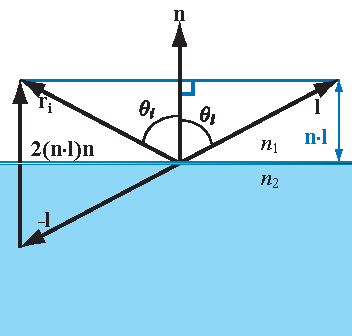
\includegraphics[height=5cm]{reflection.pdf}
    \caption{Computation of the reflection vector $\boldsymbol{r_i}$. Source:
    \autocite{RTR3}.}\label{fig:reflection}
\end{figure}

\begin{figure}[hbt]
    \centering
    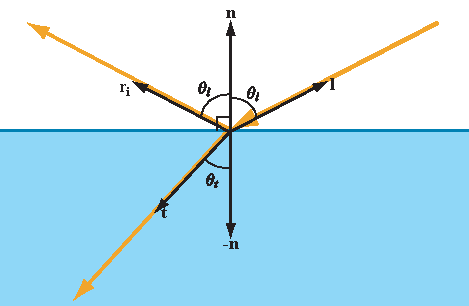
\includegraphics[height=5cm]{reflection_refraction.pdf}
    \caption{Reflection and refraction vectors $\boldsymbol{r_i}$ and
    $\boldsymbol{t}$ computed from the incoming light vector $\boldsymbol{l}$.
    Source: \autocite{RTR3}.}\label{fig:reflection_refraction}
\end{figure}

\subsubsection{Caustics}\label{subsub:caustics}

Caustics only appear in shallow water and can be observed for example in rivers,
pools, near hulls or at the beach. A caustic is formed by reflected and
refracted light rays originating from a curved surface. For real-time
applications, approximations have to be made. In
\autocite[Chapter~2]{fernando2004gpu}, Guardado and Sánchez-Crespo propose a
technique based on photon mapping using a simplified backward Monte Carlo ray
tracing method. This technique is displayed in \autoref{algo:caustics}.

\begin{algorithm}
    \small
    \DontPrintSemicolon{}
    Paint the ocean floor.\\
    For each vertex in the fine mesh:\\
    \Indp{}
        Send a vertical ray.\\
        Collide the ray with the ocean's mesh.\\
        Compute the refracted ray using Snell's Law in reverse.\\
        Use the refracted ray to compute texture coordinates for the ``Sun''
        map.\\
        Apply texture coordinates to vertices in the finer mesh.\\
    \Indm{}
    Render the ocean surface.\\
    \caption{\small{Pseudocode for real-time water caustics rendering
    \autocite[Chapter~2]{fernando2004gpu}}}\label{algo:caustics}
\end{algorithm}

Other techniques exist \autocite{darles2011survey} to compute caustics such as
in \autocite{arvo1986backward} where they are stored into an illumination map.
\citeauthor{iwasaki2001efficient} treat light rays as
``beams''\autocite{heckbert1984beam,watt1990light}. They use the Z-buffer and
stencil buffer to compute the intersection between ``illumination volumes'' and
objects. However, we think that these techniques are too costly for a
real-time application and should be simplified and computed beforehand. 

\subsubsection{Foam}\label{subsub:foam}

Foam is only formed\footnote{The other kind of foam that can be observed at
beaches is caused by the decaying of algal blooms or by pollutants and
detergents \autocite{noaa2017what}.} when the wind velocity exceeds 13km/h
\autocite{munk1947critical, darles2011survey}. In
\autocite{jensen2001deep,jeschke2003procedural} the authors use the height of
the vertex and the slope formed with the surrounding vertices to fade the foam
in and out.

Particle systems also exist to represent foam but they are too expensive to
render as many of them are needed to get realistic results
\autocite{darles2011survey}.

\subsubsection{Water Color}\label{subsub:water_color}

The color of the water depends on organic matter present in it, such as
phytoplanktons, chlorophyll concentration and turbidity.
\autocite{darles2011survey}. In \autocite{gonzato2000modelling} the authors use
a color lookup table taken from \autocite{ivanoff1972introduction} which
contains the color of the seas and oceans based on the angle between the sun and
the horizon.  \citeauthor{premovze2001rendering} use a more complicated
approach: they compute absorption and backscattering coefficients based on a
table containing the wave length of different water types
\autocite{premovze2001rendering}.  Unfortunately this method was used in a Monte
Carlo path tracer and we doubt that it can be used like this in a real-time
application.


\subsection{Methods Used in Industry Productions}\label{subsec:methods_industry}

% FFT, Projected Grid, LOD, talk about world of warships, anno, and oceans on a
% shoestring and uncharted. Talk also about some available shaders in the Unity
% store, the default one in Unity, and in Unreal Engine, also in Cryengine.

Many different water models are used in industry productions. One that has been
applied extensively in movies (such as ``Titanic'', ``13 days'', ``The World Is
Not Enough'') and most of the games is the one from Tessendorf
\autocite{tessendorf2001simulating} as seen in \cref{subsub:fft}. During our
research we came across two solutions which where presented at the Game
Developer Conference or at the SIGGRAPH conference. They are implemented in
Uncharted and World of Warships.

\subsubsection{Uncharted}\label{subsub:uncharted}

A modified version of the \textit{Wave Particle} approach from
\cref{subsub:wave_particles} has been used in \textit{Uncharted 3} (2011) and
\textit{4} (2016) to render rapids and the ocean. Developers chose this
technique because it is more intuitive for artists to control, it presents no
tiling artifacts, it is deterministic in time and fast to compute
\autocite{gonzalez2012water}. For the level of detail they use a ``Continuous
Distant-Dependent Level of Detail'' from \autocite{strugar2009continuous}. This
technique stitches quads of different size together. The quads become bigger the
further away they are from the camera. The result can be seen in
\autoref{fig:uncharted}.

\begin{figure}[hbt]
    \centering
    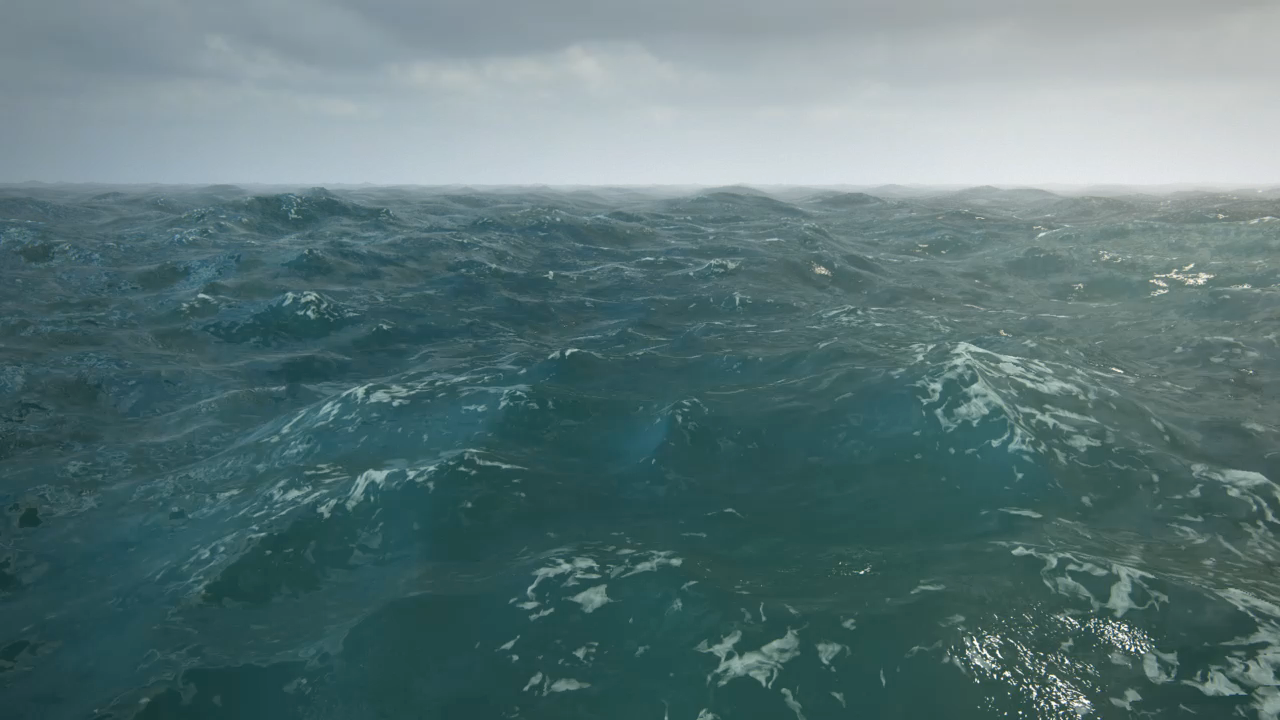
\includegraphics[height=5cm]{uncharted_ocean.png}
    \caption{View of the ocean from \textit{Uncharted 4}. Source:
    \autocite{gonzalez2016rendering}}\label{fig:uncharted}
\end{figure}


\subsubsection{World of Warships}\label{subsub:world_of_warships}

The developers at \textit{Wargaming} choose to superpose three different height
maps, as described in \autocite[Chapter~18]{pharr2005gpu}, for their
\textit{World of Warships} (2015) game \autocite{kryachko2016sea}.  For the calm
zones they use an additional one. To approximate the geometry they use the
``Projected Grid'' concept from \autocite{claes2004real}, which works as
follows:

\begin{algorithm}
    \small
    \DontPrintSemicolon{}
    Create a regular discredited plane in post-perspective space that is
    orthogonal towards the viewer.\\
    Project this plane onto a plane in the world-space.\\
    Displace the world-space vertices according to the height field.\\
    Render the projected plane.\\
    \caption{\small{Projected Grid. Source:
    \autocite{claes2004real}}}\label{algo:projected_grid}
\end{algorithm}

They took this approach because it gives them an efficient polygon distribution
over the screen \autocite{kryachko2016sea}. However, this method has several
drawbacks: it causes flickering, instability in motion, is not very accurate and
does not handle water deformations very well. By raising the triangle density up
to three to four times and redistributing them in the vertical direction, they
solved the low accuracy problem. To fix the flickering and instability in motion
issue, the developers use a modified per pixel ray casting algorithm. It
computes an improved version of Newton's method to solve the ray cast equation.
Finally they manage to create realistic water deformations with the help of six
times anti-aliasing (6xAA) \autocite{kryachko2016sea}.

\begin{figure}[hbt]
    \centering
    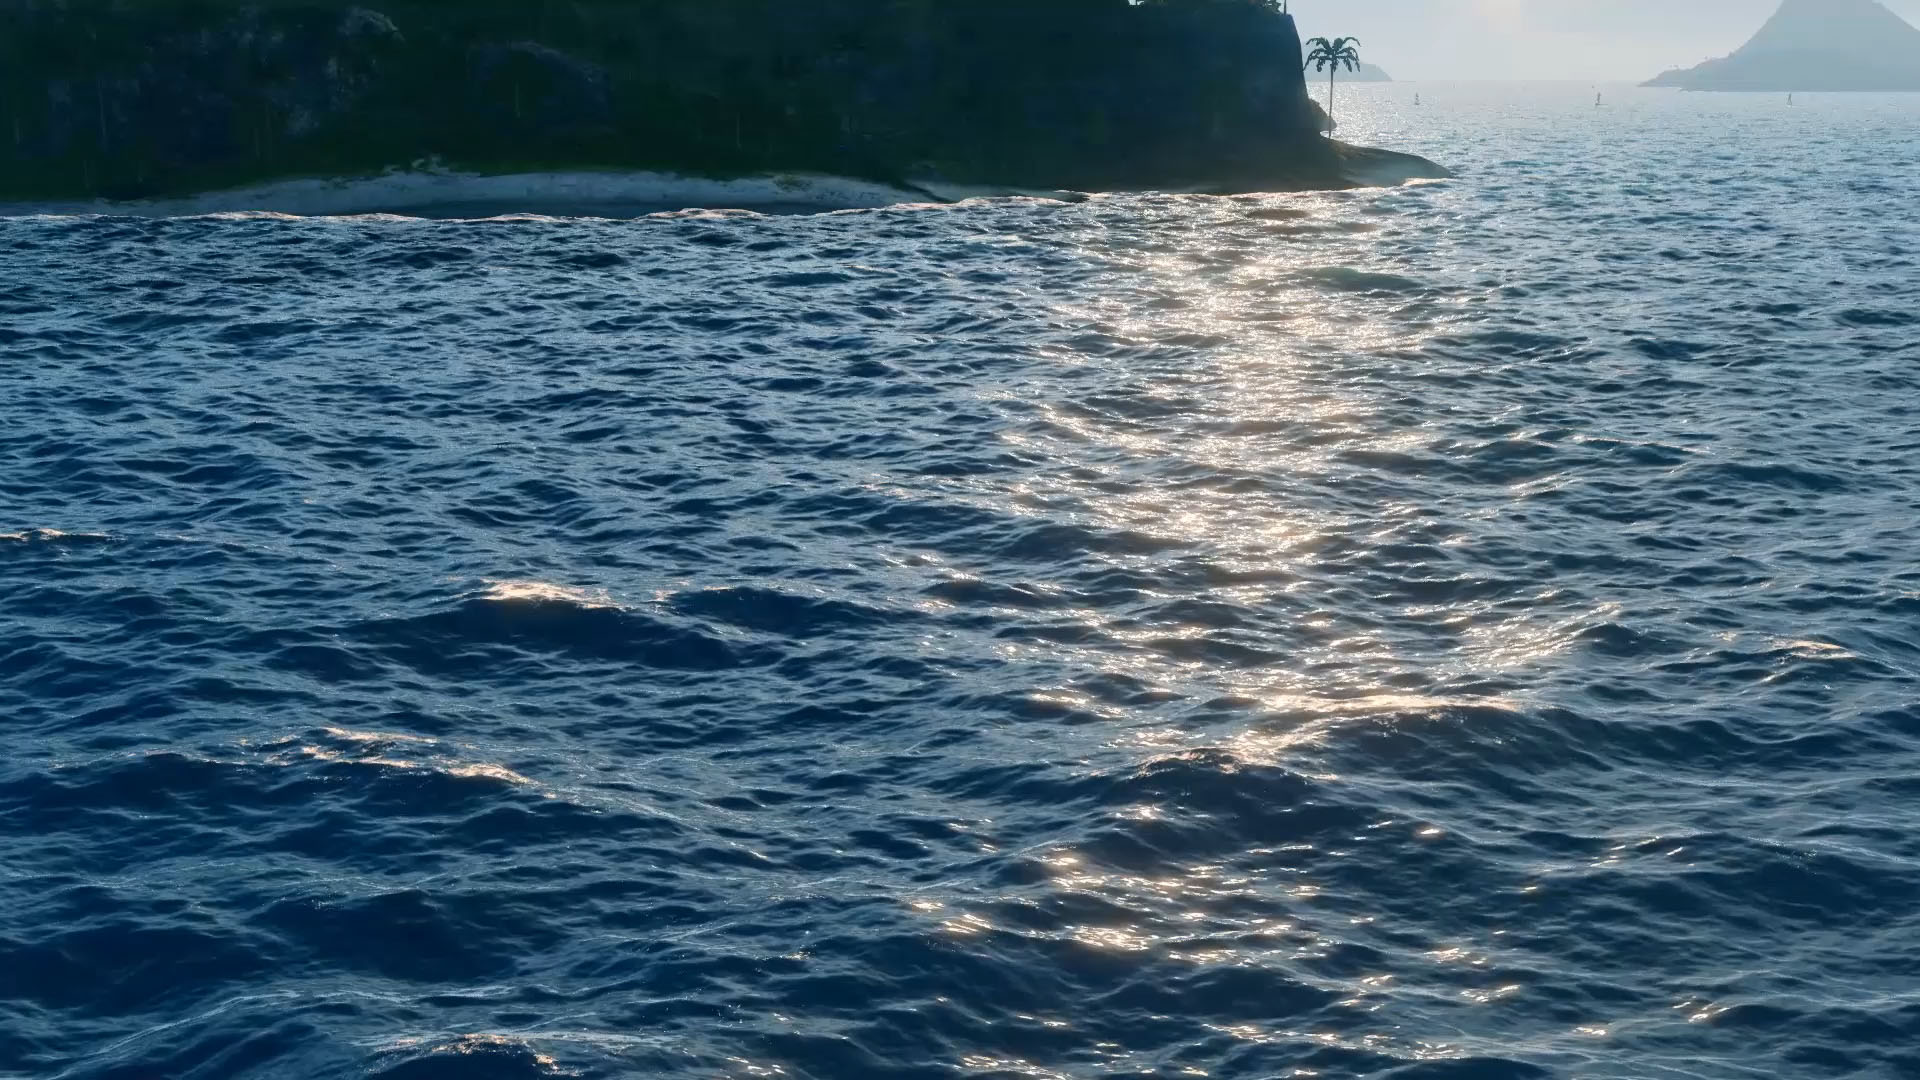
\includegraphics[height=5cm]{wow_water.jpg}
    \caption{Rendered ocean in \textit{World of Warships}. Source:
    \autocite{kryachko2016sea}}\label{fig:wow_sea}
\end{figure}

%\subsubsectjon{Undisclosed Game}\label{subsub:undisclosed_game}

\subsection{Candidate Applications for Embedding}\label{subsec:candidate_apps}

We now present two candidate applications which need a real-time water model:
\textit{SLProject} and \textit{0 A.D.} Although both have already one,
in the former application the model does not work and in the latter it is
outdated.


\subsubsection{SLProject}

\textit{SLProject} is a Scene Library developed and maintained by the cpvrLab at
the Bern University of Applied Sciences (BFH). It is free and open
source\footnote{Licensed under the GNU-GPL license.} and runs on Windows, MacOS,
Linux, Android and iOS\@. The project is a showcase for 3D computer graphics and
image processing topics such as real-time rendering, raytracing and feature
tracking. It is coded in C++ and OpenGL ES to ensure complete platform
independence \autocite{hudritch2017slproject, slproject2017doxygen}.

The project has a real-time water rendering demo but it is unfortunately broken
(see open ticket, \#36 ``Fix water
shader''\footnote{\url{https://github.com/cpvrlab/SLProject/issues/36}}). The
water plane is modeled by a simple multiplication of the sine and cosine
functions and is illuminated 50\% by a point light and 50\% by a cube texture.


\subsubsection{0 A.D.}

\textit{0 A.D.} is a real-time strategy game representing the 500 B.C to 500 A.D
era. It is developed by Wildfire Games, an independent game development studio.
The game is free, open source\footnote{Licensed under the GNU-GPL and CC BY-SA
license.} and runs on Windows, MacOS and Linux.

The development of the game began in 2000 when three modding groups whished to
create a free game engine. Up until 2009 the source code was accessible only to
members of Wildfire Games. Anyone interested in participating could make an
application and pass an interview. However, due to the fading interest of a
mod\footnote{Shorthand for the term \textit{modification}} which used 0 A.D.'s
game engine and the lack of programmers, they opened up the code in July 2009.
From then on many contributions have been made, notably one redesigning entirely
the code base, making new contributions easier. As of today the project is still
actively maintained, with the latest alpha-release (number 22 code named
``Venustas'') dating from July 26,
2017 \autocite{wildfire0adproject,wildfire0adstory}.

The game engine, Pyrogenesis, is heavily oriented towards modding. The core
engine is coded in C++ and Javascript is used for the game's logic, like the
artificial intelligence or the random generation of maps. This means that when
\textit{0 A.D.} is run, the game engine is started with a given mod. A mod
contains all the graphical elements, 3D models, sound, shaders, scenarios, map
generators and artificial intelligence.

The documentation for developers provides good build instructions, coding
conventions and codebase descriptions. Unfortunately we found that it is
difficult for a newcomer to understand the game engine architecture. It is less
documented and scattered accross multiple pages which are sometimes outadated.
The Doxygen documentation is minimalistic and unlike the one from
\textit{SLProject}, does not help to understand the architecture.

The current water implementation has been created in 2006 by a student form the
University of Waterloo, Canada, as a course project \autocite{zaharia2006cs}.
Over the years it has been slightly modified and optimized but appears visually
outdated (see \autoref{fig:0ad_water} on page~\pageref{fig:0ad_water}) compared
to the one used in commercial RTS games like Anno 1800 (see
\autoref{fig:anno}) or Age of Empires~3. There is an open ticket, \#48
``Advanced Water
Rendering''\footnote{\url{https://trac.wildfiregames.com/ticket/48}}, which was
opened twelve years ago and modified three years ago but is still not closed.
We have contacted the developers and they would gladly appreciate a contribution
that would close the issue.

\begin{figure}[hbt!]
    \centering
    \begin{subfigure}[hbt]{\textwidth}
        \centering
        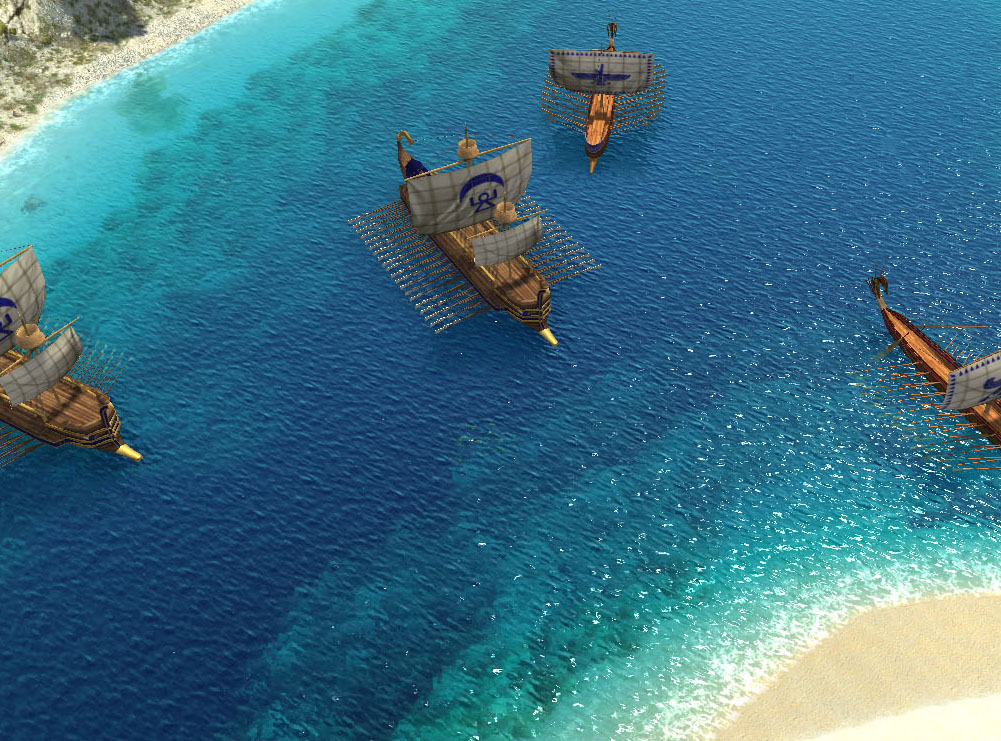
\includegraphics[height=5cm]{figures/0ad_water-specular.jpg}
        \subcaption{Close view of the water. Source:
        \url{play0ad.com}}\label{subfig:0ad_water_close}
    \end{subfigure}\\%
    %  
    \begin{subfigure}[hbt]{\textwidth}
        \centering
        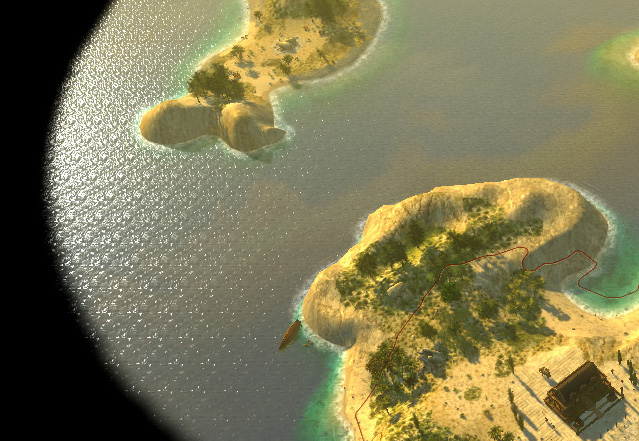
\includegraphics[height=5cm]{figures/0ad_cycladic_arcgipelago_6.jpg}
        \subcaption{Zoomed out view. Source:
        \url{play0ad.com}}\label{subfig:0ad_water_far}
    \end{subfigure}
    \caption{\textit{0 A.D.}'s water rendering. Notice on the lower left part
        of \autoref{subfig:0ad_water_close} the repetition of the waves.
        In \autoref{subfig:0ad_water_far} it is even more
    apparent.}\label{fig:0ad_water}
\end{figure}
